%% ---------------------------------------------
%%
%% Ciência da Computação - UFRPE-UAG, Brasil.
%%
%% Antônio Adelino da Silva Neto, 2019.
%% Armstrong Lohãns de Melo Gomes Quintino, 2019.
%%
%% ---------------------------------------------

\documentclass[conference]{IEEEtran}
\IEEEoverridecommandlockouts
% The preceding line is only needed to identify funding in the first footnote. If that is unneeded, please comment it out.
\usepackage{cite}
\usepackage{amsmath,amssymb,amsfonts}
\usepackage{algorithmic}
\usepackage{graphicx}
\usepackage{textcomp}
\usepackage{xcolor}

%% Usado para detectar PT-BR
% \usepackage[brazilian]{babel}

%% Usado para detectar PT-BR
\usepackage[utf8]{inputenc}

%% Usado para detectar PT-BR
\usepackage[T1]{fontenc}

\def\BibTeX{{\rm B\kern-.05em{\sc i\kern-.025em b}\kern-.08em
    T\kern-.1667em\lower.7ex\hbox{E}\kern-.125emX}}
\begin{document}

\title{Solução de baixo custo aplicado em dispositivos móveis para alerta de desastres\\
% {\footnotesize \textsuperscript{*}Note: Sub-titles are not captured in Xplore and
% should not be used}
% \thanks{Identify applicable funding agency here. If none, delete this.}
}

\author{\IEEEauthorblockN{1\textsuperscript{st} Antônio Adelino da Silva Neto}
\IEEEauthorblockA{\textit{Bel. em Ciência da Computação} \\
\textit{Universidade Federal Rural de Pernambuco}\\
Garanhuns, Brasil \\
antonio.asn03@gmail.com}
\and
\IEEEauthorblockN{2\textsuperscript{nd} Armstrong Lohãns de M. G. Quintino }
\IEEEauthorblockA{\textit{Bel. em Ciência da Computação} \\
\textit{Universidade Federal Rural de Pernambuco}\\
Garanhuns, Brasil \\
lohansdemelo1108@gmail.com}
}

\maketitle

\begin{abstract}
Occurrences of human and natural disasters are increasingly common today, regardless of location, all humans are susceptible to suffer any damage from them, so a disaster warning channel becomes even more important. This paper presents a prototype disaster warning system in a simple and precise way, focusing on the possibility of warning of imminent danger in a given area, with the help of the use of the system by the population. The research for the development of the idea is based on the study of the literature about mobile transmission systems, in order to find the best result for application of the system.
\end{abstract}

\begin{IEEEkeywords}
disaster, mobile system, danger alert.
\end{IEEEkeywords}

\section{Introduction}
Dentre as inúmeras alterações ocorridas no planeta nas últimas décadas, grande parte delas causadas em decorrência de efeitos estimulados diretamente ou indiretamente por ações antropológicas, é de se destacar a importância do estudo dessas mudanças. Tal estudo mostra-se como uma condição necessária para o desenvolvimento futuro da sociedade humana, bem como pesquisas a fim de achar soluções emergenciais para problemas vinculados a essas condições.

Tais mudanças planetárias são responsáveis por desastres naturais que causam uma enorme perda financeira e humana para a sociedade, um exemplo prático e comum desses desastres no contexto nacional são as enchentes, as quais trazem um enorme transtorno e perdas para as comunidades afetadas [3] além de inúmeros outros exemplos globais, como terremotos, queimadas e tsunamis. 

Partindo desses fatos, é de grande notoriedade a importância da busca por soluções emergenciais para problemas relacionados a desastres naturais e desastres em um modo geral.  

Considerando também o recente avanço das tecnologias da informação de modo geral e especialmente a popularização do uso de dispositivos móveis, além do aumento da capacidade e da qualidade de conexão entre esses equipamentos, é de se pensar que problemas causados pela ocorrência de desastres possam ser remediados a partir de aplicações que envolvam os dispositivos móveis.

Um exemplo do uso de dispositivos móveis em desastres pôde ser visto durante o maremoto que atingiu, no final de dezembro de 2004, alguns países da Ásia e da África, nas quais as tecnologias móveis (principalmente o uso de redes móveis como o Wi-fi e o SMS), romperam barreiras geográficas e ajudaram inúmeras vítimas. Estas tecnologias foram de imensa importância  para encontrar desaparecidos e para auxiliar as vítimas que precisavam de socorro [5].

Partindo desses parâmetros e levando em consideração a crescente evolução dos dispositivos móveis, pode-se afirmar que remediação de desastres vem por intermédio de estudos tecnológicos, os quais devem ter como objetivo a minimização e a diminuição dos impactos destes desastres na sociedade [4]. 

Dessa forma, o presente artigo busca descrever a implementação de uma aplicação para o sistema operacional Android voltada para o compartilhamento de mensagens em meio a desastres naturais ou ocasionais, tendo em vista que muitas vezes esses desastres provocam a destruição da infra-estrutura de telecomunicações local, causando sérios problemas para a equipe de resgate resgate [6] e para toda a população local.

Esse aplicativo utiliza-se da conexão Bluetooth dos aparelhos móveis para que as mensagens de alerta ou semelhantes sejam compartilhadas de aparelho em aparelho (como uma espécie de conexão par a par) tendo a finalidade de informar as demais pessoas da população sobre o desastre ocorrido, além de poder ser usado para o auxílio imediato às vítimas do desastre com informações ágeis. Assim podendo gerar uma comunicação simples, rápida e barata entre as pessoas em meio a um ambiente caótico de desastres.

\section{Trabalhos Relacionados}

Na literatura existem inúmeras pesquisas relacionadas a sistemas de alerta de desastres e de emergência, entretanto em um contexto geral os trabalhos encontrados na literatura analisam, discutem e implementam maneiras de fazer o sensoriamento de áreas de risco e emitir alertas com base em dados obtidos por estes sensores. Foram encontrados também trabalhos relacionados a comunicação por dispositivos móveis em desastres e temas semelhantes. Por fim, listamos como o trabalhos mais relevantes para a elaboração do presente estudo os listados e brevemente detalhados abaixo.

\subsection{Artigo A}

Pesquisadores brasileiros buscaram em sua pesquisa avaliar se as informações compartilhadas nas redes sociais a respeito de possíveis eventos críticos conferem subsídios para investigar, planejar, monitorar ameaças  e  avaliar  os  riscos  para que se possa empregar  os  recursos necessários para a prestação de socorro de  forma  efetiva. A comunicação entre instituições, profissionais e população oportuniza uma rede de ligações para a cooperação de recursos. Essa cooperação possibilita a mobilização desses recursos para seu emprego em emergências ou eventos críticos. As redes sociais online podem vir a favorecer esta cooperação entre civis e instituições responsáveis. O objetivo do trabalho desses pesquisadores foi estudar as redes sociais online, com foco no Twitter, para identificar as oportunidades e os riscos em seu uso na comunicação em emergências e eventos críticos atendidos pelo Corpo de Bombeiros Militar de Santa Catarina (CBMSC). Os resultados dessa pesquisa permitem constatar que o CBMSC tem dificuldades na interação com a sociedade e outras instituições e destacam a importância benéfica da interação instituição-sociedade diante de eventuais desastres [2].

\subsection{Artigo B}

Pesquisadores chineses, apresentam um estudo que toma como base a ocorrência frequente de doenças artificiais e desastres naturais, detalham eu seu estudo um sistema de comandos e respostas de emergência baseado em dispositivos móveis, incluindo detalhes do projeto do módulo de função. O sistema citado cria um plataforma de comando e resposta móvel de emergência com a função de liberar e coletar informações importantes em um cenário de desastres. A aplicação mostra-se favorável à promoção de processos rápidos e eficientes em situações emergenciais. Os funcionários que prestam serviços de atendimento às vítimas no local podem receber uma mensagem precisa sobre o evento além de possibilitar a instituição de tomada de decisão responsável um posicionamento mais concreto e objetivo o que pode vir a gerar diretrizes importantes para que o trabalho da equipe de resgate seja guiado por essas pelas informações coletadas [7].

\subsection{Artigo C}

Em artigo de pesquisadora brasileira publicado pela Brazilian Journal of Technology, Communication, and Cognitive Science, descreve como objeto da pesquisa a avaliação de aplicativos voltados a desastres naturais, para isso foram avaliados aplicativos (doravante apps) de comunicação e prevenção de riscos e desastres disponíveis em sistema operacional Android em todas as versões, verificando também a plataforma da AppStore disponível para os dispositivos com sistema operacional IOS em todas as versões. Buscando assim identificar o número e o perfil dos aplicativos disponíveis para os cidadãos brasileiros e em língua portuguesa, entretanto a pesquisa também incluiu aqueles disponíveis em língua inglesa, a despeito do potencial de uso mais restrito. O estudo do perfil dos aplicativos buscou avaliar a importância do mobile learning no processo de mitigação e preparação de um desastre [1].

\subsection{Artigo D}

Pesquisadores da Universidade de Twente, Países Baixos, apresentam um estudo que artigo gira em torno do conceito de 
utilizar os modernos recursos de comunicação de smartphones para transmitir mensagens através de uma rede ad hoc 
durante um desastre, que torna inacessível a estação base celular tradicional. Devido a natureza dinâmica e 
descentralizada do ambiente considerado, algoritmos epidêmicos se apresentam como uma opção adequada para 
divulgação de mensagens. Eles consideraram um cenário específico para propor um protocolo de roteamento 
epidêmico modificado que possa ser útil durante desastres naturais. Desenvolveram então uma ferramenta 
de simulação usando MATLAB para avaliar a influência de vários fatores no desempenho e custo de no protocolo 
de roteamento epidêmico modificado em caso de emergência [6].\newline

Os artigos trabalhados acima citados estão intimamente vinculados ao presente estudo, abaixo está presente uma 
tabela comparativa (Tabela 1) entre os quatro artigos anteriormente citados, as colunas da tabela correspondem 
aos critérios de avaliação dos trabalhos e as linhas correspondem aos trabalhos acima enumerados.

%  PNG ruim
% \begin{figure}[htbp]
% \centerline{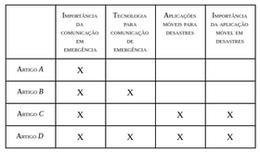
\includegraphics{tabela1.png}}
% \caption{Tabela Comparativa de Trabalhos Relacionados}
% \label{fig}
% \end{figure}

\begin{table}[htbp]
\caption{Tabela Comparativa de Trabalhos Relacionados}
\begin{center}
\begin{tabular}{|c|c|c|c|c|}
\hline
% \textbf{Table}&\multicolumn{3}{|c|}{\textbf{Table Column Head}} \\
% \cline{2-4} 
\textbf{Artigos} & \textbf{\textit{Informação$^{\mathrm{1}}$}}& \textbf{\textit{Informação$^{\mathrm{2}}$}}& \textbf{\textit{Informação$^{\mathrm{3}}$}}& \textbf{\textit{Informação$^{\mathrm{4}}$}}  \\
\hline
Artigo A & X &  &  &  \\
\hline
Artigo B & X & X &  &  \\
\hline
Artigo C & X &  & X & X  \\
\hline
Artigo D & X & X & X & X \\
\hline

\multicolumn{4}{l}{Legenda:}\cr
\multicolumn{4}{l}{$^{\mathrm{1}}$Importância da comunicação em emergência.}\cr
\multicolumn{4}{l}{$^{\mathrm{2}}$Tecnologia para comunicação de emergência}\cr
\multicolumn{4}{l}{$^{\mathrm{3}}$Aplicações móveis para desastres.}\cr
\multicolumn{4}{l}{$^{\mathrm{4}}$Importância da aplicação móvel em  desastres}\cr
\end{tabular}
\label{tab1}
\end{center}
\end{table}

% \begin{table}[htbp]
%     \centering
%     \begin{tabular}{lllll}
%      & Importância da comunicação em emergência & Tecnologia para comunicação de emergência & Aplicações móveis para desastres & Importância da aplicação móvel em  desastres \\
%     \begin{tabular}[c]{@{}l@{}}Artigo \\ A\end{tabular} & X &  &  &  \\
%     \begin{tabular}[c]{@{}l@{}}Artigo \\ B\end{tabular} & X & X &  &  \\
%     \begin{tabular}[c]{@{}l@{}}Artigo \\ C\end{tabular} & X &  & X & X
%     \end{tabular}
%     \end{table}

\section{Proposta}

O primeiro passo a ser abordado é o cenário onde esse sistema poderá ser implementado, para que em seguida possamos interpretar como a implementação será feita e  assim poderemos analisar as consequências da utilização do mesmo.

\subsection{Cenário}\label{AA}
Quando analisamos o histórico de tragédias relacionadas a desastres naturais no Brasil, o qual não é mais uma surpresa que esteja exposto a uma variedade de perigos naturais, temos a recordação recente do aumento no número de casos por todo o país, um breve lembrança: Enchentes e deslizamentos na Região Serrana do Rio de Janeiro (janeiro de 2011), rompimento da barragem em Mariana (5 de novembro de 2015), rompimento da barragem em Brumadinho (25 de janeiro de 2019), chuva forte com enchentes no Rio de Janeiro  (8 de abril de 2019), queimadas e focos de incêndio na amazônia (29 de setembro de 2019).

A maior parte dos desastres naturais são decorrentes de eventos climáticos como seca, chuvas fortes e deslizamentos de terra. 

Enquanto as regiões Norte e Nordeste do país sofre em sua maior parte com as secas e queimadas, o Sul  e Sudeste do Brasil são afetados constantemente por chuvas muito abundante, ventos e granizo. Tornando o Brasil exposto a uma grande diversidade de eventos naturais que representam um árduo desafio para os governos e a população.

\subsection{Ideia da implementação}

Analisando estes fatos, que vem ocorrendo com mais frequência desde a última década, um país como o Brasil, de vasta extensão territorial, carece de soluções que agregam às medidas políticas aplicadas em seu território, então, um sistema móvel que fosse capaz de alertar a população e seus governantes sobre o risco iminente de uma tragédia seria de grande utilidade, visto que a aplicação do mesmo auxiliaria na transmissão de emergência e ajudaria a combater com antecedência casos fatais provenientes das tragédias.

\section{Considerações finais}

Após um período de estudos, temos como conclusão parcial que é possível montar um sistema que consegue alertar focos de desastres de forma funcional e de baixo custo, futuramente tornando-se pronto para ser expandido a um sistema completo e de fácil implementação. O maior obstáculo encontrado porém, foi a forma de implementação da comunicação, o qual deverá ser feita inicialmente via rede wifi ou bluetooth.

% \section*{Referências}

\begin{thebibliography}{00}
\bibitem{b1} da Silva, Ariana Moura, and Margarethe Born Steinberger-Elias. "Educação, Tecnologia e Comunicação de Desastres com Dispositivos Móveis." Anais do Encontro Internacional Tecnologia, Comunicação e Ciência Cognitiva 2.1 (2016).
\bibitem{b2} Pratts, André Luís Hach, and Douglas Tomaz Machado. "Redes sociais online no CBMSC: seu emprego como meio de comunicação em emergências e eventos críticos." Revista Ordem Pública 9.1 (2016): 51-66.
\bibitem{b3} de Lima, Andressa SA, et al. "Aplicativo colaborativo para alerta de vulnerabilidade a alagamentos e enchentes no Vale do Itajaí." 9º Workshop de Computação Aplicada a Gestão do Meio Ambiente e Recursos Naturais. Vol. 9. SBC, 2018.
\bibitem{b4} Hsiao, Edward, et al. "Implementação em Hardware de uma Rede de Sensores para Monitoramento e Alerta de Desastres Naturais." Anais do I Workshop de Computação Urbana (COURB 2017). Vol. 1. No. 1/2017. SBC, 2017.
\bibitem{b5} LEMOS, André; NOVAS, Lorena. “Cibercultura e tsunamis: tecnologias de comunicação móvel, blogs e mobilização social.” Revista FAMECOS: mídia, cultura e tecnologia, n. 26, p. 29-40, 2005.
\bibitem{b6} Wu, Xian, et al. "Emergency message dissemination system for smartphones during natural disasters." 2011 11th International Conference on ITS Telecommunications. IEEE, 2011.
\bibitem{b7} Yin, Bo, et al. "Research and design of an emergency command system based on mobile devices." Proceedings of 2011 International Conference on Electronic \& Mechanical Engineering and Information Technology. Vol. 5. IEEE, 2011.
\bibitem{b8} PEDROSO, F., and N. HOLM-NIELSEN. "Desastres naturais no Brasil: Um ciclo de tragédias anunciadas." Nexo. Disponível em: https://www. nexojornal. com. br/ensaio/2017/Desastres-Naturais-no-Brasil-um-ciclo-de-tragédias-anunciadas. Acesso em 3 (2018).
\end{thebibliography}
\vspace{12pt}
% \color{red}
% IEEE conference templates contain guidance text for composing and formatting conference papers. Please ensure that all template text is removed from your conference paper prior to submission to the conference. Failure to remove the template text from your paper may result in your paper not being published.

\end{document}

% \bibitem{b3} de Lima, Andressa SA, et al. "Aplicativo colaborativo para alerta de vulnerabilidade a alagamentos e enchentes no Vale do Itajaí." 9º Workshop de Computação Aplicada a Gestão do Meio Ambiente e Recursos Naturais (WCAMA_CSBC 2018). Vol. 9. SBC, 2018.
% \bibitem{b4} Hsiao, Edward, et al. "Implementação em Hardware de uma Rede de Sensores para Monitoramento e Alerta de Desastres Naturais." Anais do I Workshop de Computação Urbana (COURB 2017). Vol. 1. No. 1/2017. SBC, 2017.
% \bibitem{b5} LEMOS, André; NOVAS, Lorena. “Cibercultura e tsunamis: tecnologias de comunicação móvel, blogs e mobilização social.” Revista FAMECOS: mídia, cultura e tecnologia, n. 26, p. 29-40, 2005.
